	\chapter{Odds And Ends}
There is, of course, never enough time to talk about all the topics that one would want to. Here are a few lectures which don't really sit on the main course of the class, but are pleasant explorations in side topics of combinatorial topology. These topics also occurred frequently enough as prerequisite knowledge for a number of projects that it seems like a good idea to include them as short references for projects, or perhaps as samples for what a project should feel like. 
\newpage

\section{Sperner's Lemma}
	We digress for a moment to talk about the 2 dimensional case of Sperner's lemma, which discusses colorings of triangulations. A triangulation is a network of vertices and edges, where every face of this network is a triangle. 
	\begin{theorem}[Sperner's Lemma]
	Let $T$ be a triangulation of $x+y+z=1$ with $x, y, z\geq 0$ with labeled vertices $t_{xyz}$. Suppose each vertex is colored either red, green or blue in such a way that 
	\begin{itemize}
	\item If $x=0$, then $t_{xyz}$ is not colored red
	\item If $y=0$, then $t_{xyz}$ is not colored blue
	\item If $z=0$, then $t_{xyz}$ is not colored green
	\end{itemize}
	Then there exists a small triangle in the triangulation, $\Delta$ that has the color of all three vertices different.
	\end{theorem}
	\begin{proof} 
	We will call the small triangles $\Delta$ rooms, which we will usually identify with their bottom left corner.
	We add a ``door'' to the edge in the array $T$ if the vertices that bound the edge are blue and red. Then all rooms with just 1 door have all different colors for vertices. Every other room has either no doors or 2 doors. 
	By construction, one side of $T$ contains only blue and red vertices. If a door separates the interior and the exterior of $T$, then it must lie on this blue-green side.
\[
         Sperners!%       \includegraphics[scale=.4]{SpernerPath}
\]
	\begin{exercise}
	Prove that there an odd number of doors that separate the interior of $T$ to the exterior of $T$.
	\end{exercise}
	For each door on the boundary of $T$, construct a path that travels through $T$ by going through doors, and only going through a door once. This process uniquely determines a path for each initially selected door. This path either terminates in $T$, or it at some point leaves $T$ through another door. As each path that can both enter and leave $T$ uses 2 boundary doors, there must be a path that is unable to leave $T$, as the number of doors on the boundary of $T$ is odd. This implies that a path gets "stuck" in $T$, i.e. it moves into a room with just 1 door. This implies the existence of a red-green-blue room.
	\end{proof}

Using Sperner's Lemma, we prove Brower's fixed point theorem. 
\begin{theorem}[\cite{brouwer1911abbildung}].
Every continuous function $f: D^2\to D^2$ fixes some point. 
\end{theorem}
\begin{proof}
We first prove that there is no function $g: D^2\to \partial D$ that acts as the identity on $\partial D$. Take a triangulation of $D^2$, and divide $\partial D$ into three components: Red, green, blue. Then a map $g:D^2\to \partial D$ gives a coloring to any triangulation of $D^2$. By Sperner's lemma, there must be a RGB triangle. This means that the vertices of the triangle are mapped to the Red, Green and Blue components respectively. This is impossible, as  the map is suppose to be continuous (and therefore uniformly continuous), but an arbitrarily small triangle is mapped to a set of large size.\\
With this, it is easy to prove that every function $f: D^2\to D^2$ fixes a point. We prove by contradiction. Suppose that $f$ is a function that has no fixed points. Then define a new function,  $H(x,  t): [0, 1]\times D^2\to D^2$ by the following method:
	\begin{itemize}
		\item Suppose that you want to know $H(x,  t)$. Draw the points $x$ and $f(x)$.
		\item Draw a line from $f(x)$ through $x$. This hits a unique point on the boundary of the circle.
		\item Define $H(x, t)$ to be that point which is $100\cdot t\%$ along the line that you have just drawn. 	When $t=0$,  this should be the identity. When $t=1$,  $H(x,  t)$ always gives a point on the boundary circle. 
	\end{itemize}
	Notice that the second step in this definition crucially uses the fact that $f(x)\neq x$ for all $x$. Additionally,  $h(x)$ is a continuous function. Finally,  notice that $H(x, t)$ is a deformation retract to the boundary of the disk. However,  we know that there is no deformation retract of the disk to the circle; this is a contradiction! 
\end{proof}

This theorem is 


\subsection{Nash Equilibria}
Nash Equilibria is a method that you can apply to mixed strategy problems.
\begin{definition}
	A \emph{strategy game} between $k$ players is the following pieces of data:
	\begin{itemize}
		\item For every player $i$,   a non-empty finite set $S_i$ of \emph{strategies}.
		\item For every player $i$,  a continuous function $P_i: S_1\times S_2\times  S_k\to \R$ called the \emph{payoff} function,  which assigns to each possible combination of strategies played,  the payoff of player $i$. 
	\end{itemize}
\end{definition}
\begin{definition}
	A \emph{set of mixed strategies} for $k$ players is a function $\Sigma: S_1\times S_2\times S_k\to \R$ where $\sum_{s\in S_k} f(s)=1$. The set of all mixed strategies denoted to $\mathbb D$. 
\end{definition}
\begin{definition}
	A \emph{Nash Equilibrium} is a set of mixed strategies $x\in \mathbb D$ where each player cannot improve their utility by changing their specific strategy (with all other players' strategies kept the same). 
\end{definition}

Notice that the set of mixed strategies is homeomorphic to $D^{|S_1|}\times \cdots \times D^{|S_k|}\cong D^{|S_1|+\cdots +|S_k|}$. 
\begin{definition}
	Given a mixed strategy $\Sigma$,  we define the expected payoff of $\Sigma$ to be 
	\[\mathbb{E}(\Sigma):= (\sum_{s\in S_1} \Sigma(s) P_1 (s),  \sum_{s\in S_2} \Sigma(s) P_2(s),  \ldots,  \sum_{s\in S_k} \Sigma(s) P_k(s))\]
	This expected payoff function is a continuous function from the set of mixed strategies to the set of all payoffs,   $\mathbb D \to \R^k$. 
\end{definition}
\begin{definition}
	Given a mixed strategy $\Sigma$,  define the \emph{Best Response of player $i$} of $\Sigma$ to be the subset of $D^{|S_i|}$ which maximizes player $i$ payoff,  assuming all of the other players maintain the same strategy.\\
	Given a mixed strategy $\Sigma\in \mathbb D$,  define the \emph{updated strategy} to be the subset $Up(\Sigma)$ where every player has replaced their strategy with a Best Response. 
\end{definition}

\begin{claim}
	Let $\Sigma \in \mathbb D$ be a mixed strategy. If $\Sigma\in Up(\Sigma)$,  then $x$ is a Nash Equilibrium point. 
\end{claim}
\begin{proof}
	Check the definitions. 
\end{proof}
\begin{theorem}
	Every mixed strategy game has a Nash Equilibrium. 
\end{theorem}
\begin{proof}
	We have the update strategy function that takes a mixed strategy $\Sigma\in \mathbb D$ and replaces it with the set of mixed strategies that are the best possible response. This set is convex. Define the average mixed strategy to be the average of $Up(\Sigma)$. We will denote this as 
	\[\widetilde{Up}(\Sigma)\]
	Now,  $\widetilde{Up}(\Sigma)$ is a function from $\mathbb D\to \mathbb D$. Since $\mathbb D$ is homeomorphic to a disk,  this function must have a fixed point. This fixed point has the property that $x=\widetilde{Up}(x)\subset Up(x)$. So this gives us a Nash Equilibrium.
\end{proof}
\newpage

\section{Posets and Simplicial Complexes}

\begin{definition}
A \emph{partially ordered set}, or \emph{poset} for short, is a set $P$ with an order relation $\leq$ satisfying the properties of transitivity, reflexivity, and antisymmetry.
\end{definition}
The reason that a poset is partially ordered is that it may not be possible to compare any given pair of elements in that poset. 
\begin{example}
 The sets $\mathbb N,  \mathbb Z,  \mathbb Q,  \mathbb R$ are all posets with the standard ordering.\\
  A more interesting way to order the set $\N$ is with the order $\leq_|$,  which says that $a\leq_|b$ if $a$ divides $b$. For example,  $3\leq_|6$,  but $3\not\leq_|7$. Notice that not every pair of elements are compatible in this partial ordering on $\N$. 
\end{example}
The structure of a partial order is still enough to carry over many of the constructs from a full order. 

\begin{definition}
	Let $(P,  \leq)$ be a poset,  and $a\leq b\in P$. 
	\begin{itemize}
		\item Define the \textbf{closed interval}$[a, b]$ to be the set of all elements greater than or equal to $a$,  and less than or equal to $b$. 
		\[ [a, b]:=\{p\in P\;|\;a\leq p\leq b\}\]
		\item We say that $a$ \textbf{is covered by} $b$ ( or $b$ \textbf{covers} $a$) if the interval $[a, b]$ contains only 2 elements. In this case we write $a\lessdot b$.
	\end{itemize}
\end{definition}
It will oftentimes be convenient to encode the information of a poset graphically. 
\begin{definition}
	Let $(P,  \leq)$ be a finite poset. The \textbf{Hasse Diagram} of $P$ is a diagram with vertices given by the elements of $P$,  and an edge drawn \emph{upward} from a vertex $a$ to a vertex $b$ if $a\lessdot b$.
\end{definition}
Hasse diagrams are much easier to understand if you've seen a couple examples. Here are the Hasse diagrams for a few familiar posets.
For us,  it will oftentimes be convenient to encode the information of a poset pictorially. 
\begin{definition}
	Let $(P,  \leq)$ be a finite poset. The \textbf{Hasse Diagram} of $P$ is a diagram with vertices given by the elements of $P$,  and an edge drawn \emph{upward} from a vertex $a$ to a vertex $b$ if $a\lessdot b$.
\end{definition}
Hasse diagrams are much easier to understand if you've seen a couple examples. Here are the Hasse diagrams for a few familiar posets.
\begin{example}
	\begin{itemize}
		\item Look at the poset $[0, 4]$ with the usual ordering. This has a Hasse diagram that looks like this:
		\[\begin{tikzcd}
		  	4\arrow[dash]{d} \\3\arrow[dash]{d} \\2\arrow[dash]{d} \\1\arrow[dash]{d} \\0
		  \end{tikzcd}\]
		\item Look at the numbers between $0$ and $12$ with the ordering $a\leq_|b$ if $a$ divides $b$. This has a Hasse Diagram
		\[
			\begin{tikzcd}
				\;& 12& 8\\
				9&6 \arrow[dash]{u}&4\arrow[dash]{ul} \arrow[dash]{u} & 10\\
				3\arrow[dash]{u} \arrow[dash]{ur} &2 \arrow[dash]{ur} \arrow[dash]{u} \arrow[dash]{rru} &5 \arrow[dash]{ru} &7&11\\
				&&1 \arrow[dash]{ull} \arrow[dash]{ul} \arrow[dash]{u} \arrow[dash]{ur} \arrow[dash]{urr}
			\end{tikzcd}
		\]
		\end{itemize}
\end{example}
The primary example that we will be working with is the poset associated to a simplicial complex.
\begin{definition}
 Given $\Delta$ a simplicial complex, we construct a poset $P(\Delta)$ which
 \begin{itemize}
 \item As a set, has elements $\Delta\setminus\{\emptyset\}$
 \item Has order relation  $\sigma_1\leq \sigma_2$ in $P(\Delta)$ if $\sigma_1\subset \sigma_2$. 
 \end{itemize}
\end{definition}

What properties do all of these Posets have?
\begin{definition}
 A \emph{simplicial poset} is a poset with a minimal element $\hat 0$ with the property that for all $x\in P$, the interval $[0, x]$ is isomorphic as a poset to some Boolean poset $B_n$. 
\end{definition}
It is clear that not every poset is a simplicial poset.
\begin{claim}
Simplicial posets are the same as abstract simplicial complexes.
\end{claim}
To every poset, we can associate a \emph{order complex} to it, which consists of all chains in the poset. We denote this simplicial complex as $\Delta(P)$. \\ If $P$ is a poset with a minimal element, let $\bar P$ be the poset missing that minimal element. 



\subsection{The Incidence Algebra}
One thing that is particularly interesting to us are functions that assign a value to every interval of a poset. For instance,  given a poset $P$,  consider the function that assigns to the interval $[a, b]$
\[f([a, b])=\text{number of elements in }[a, b]\]
\begin{definition}
	Let $P$ be a finite poset. Define the \textbf{Incidence algebra} to be the set of functions of the form
	\[f:\{a\leq b\}\to \R.\]
	Given two such functions $f$ and $g$, we can build a new function $f*g\in I(P)$. To define $f*g$,  we need to say what it's value is on every interval:
	\[f*g([a, b])=\sum_{a\leq c\leq b} f([a, c])g([c, b]).\]
\end{definition}
There are a few special functions that belong to every incidence algebra. 

\begin{example}
	 Let's look at $\mathcal P(\underbar 3)$,  the poset of subsets of $\{1, 2, 3\}$. 
	 \begin{itemize}
	 	\item The \textbf{counting function} $c([a, b])$ takes value equal to the number of elements in the interval $[a, b]$. For example
	 	\[c([\{1, 2, 3\},  \{1\}])=4.\]
	 	\item The \textbf{$\delta$ function} $\delta([a, b])$  takes a value of $1$ if $a=b$,  and $0$ otherwise. 
	 	\[\delta([\{1\},\{1, 2\}])=0\;\;\;\;\; \delta([\{2\}, \{2\}])=1)\]
	 	The \textbf{$\delta$-function} has the property that for every other $f\in I(P)$,  
	 	\[\delta*f=f.\]
	 	\item The $\zeta$-function takes a value of $1$ on every interval.
	 	\[\zeta([\{1\}, \{1, 2, 3\}])=1\]
	 	\item The \textbf{M\"obius function} is the unique function $\mu$ that has the property that 
	 	\[\mu*\zeta=\delta.\]
	 	On the poset $\mathcal P(\underbar 3)$,  this is given by 
	 	\[\mu([U,  V])=(-1)^{|V|-|U|}\]
	 	\item The \textbf{covering function} $\eta([a, b])$ assigns $1$ if $a\lessdot b$ and $0$ otherwise. 
	 	\[\eta([\{1\},\{1, 2\}])=1\;\;\;\;\; \eta([\{2\}, \{2\}])=0)\]
	 \end{itemize}
\end{example}
\begin{lemma}
	We can directly define the M\"obius function recursively as follows:
	\[
		\mu(x, y)=\left\{\begin{array}{cc}
		                 	1 & \text{if $x=y$}\\
		                 	-\sum_{x\leq z < y} \mu(x,  z) & \text{for $x<y$}\\
		                 	0 & \text{otherwise}
		                 \end{array}	\right.\]
\end{lemma}
\begin{proof}
	Exercise!
\end{proof}
\begin{definition}
	A \textbf{chain} of $P$ is a sequence of element in $P$ \[a_1<a_2<\cdots a_{n-1}< a_n.\]. 
\end{definition}

\begin{lemma}
	Suppose that $P$ is a poset that has a largest and smallest element (which we will denote $\hat 0$ and $\hat 1$. Then $\mu(\hat 0,  \hat 1)=-c_1+c_2-c_3+\ldots (-1)^r c_r$,  where $c_r$ is the number of chains of length $r$. 
\end{lemma}



\begin{theorem}
	Suppose that $P$ is a poset. Further suppose that $P$ has a largest and smallest element,  which we will call $\hat 0$ and $\hat 1$. . Then $P^c$ is a simplicial poset,  at we have that 
	\[\chi(P^c)-1=\mu(\hat 0,  \hat 1).\]
\end{theorem}


\newpage
\section{Braids}
\label{sec:knot:braids}
Braid groups describe one particular way that we can tangle stings together. Intuitively, a braid is a tangle of strings that go from top to bottom, that is they proceed in only one direction. The stings of the braid can't intersect, and they can't loop back on themselves. A braid is like a permutation with some additional information encoded about the order that you took the permutations in, and we will formally see later why this is an accurate description of the braid group.
\begin{definition} A collection of functions $f_i:[0,1]\to \RR^3$ , $i\in {1,2,\ldots n}$ is called a \textbf{braid on $n$ strings} and is written as $\beta$ if the following properties hold:
\begin{enumerate}
\item $f_i(x) \in \{x\}\times \RR^2$
\item $f_i(x)\neq f_j(x)$ for all $i\neq j$
\item $\im f_i$ is a finite collection of line segments
\item $f_i(0)=(i,0,0) $ and $f_i(1)=(\sigma(i),0,1)$ where $\sigma_i\in S_n$ a permutation function.
\end{enumerate}
\end{definition}

\[
BRAIDS?
\]


As one can see, this definition says that a braid is much like a knot, in that it can be represented by a finite collection of line segments, and that it does not intersect itself. How a braid is different than a knot (or a link) is that braids ``travel" in one direction, that is, if we orient the braid by the orientation $[0,1]$, we see that the image of the braid is oriented against a single axis. We will choose this axis to be the $x$ axis, and hence going along the braid means ``going left to right." Like knots, we are interested in braids up to the equivalence of ambient isotopy; when we draw a braid, we really are just picking a representative of the equivalence class of braids on $n$
strings that are isotopic to this one. We will denote the set of all equivalence classes of braids with $n$ strings as $\mathcal{B}_n$. Here are some equivalent braids.
\[
A BRAID
\]


How can we make a group out of braids? The way that designed our braids, we can form a group operation by braid ``stacking'', that is placing one braid on top of each other. 

\begin{definition} Let $\beta_1, \beta_2\in \mathcal{B}_n$, where $\beta_1=\{f_i(t)\}$ and $\beta_2=\{f_i'(t)\}$. Define the new braid $\beta_3=\{g_i\}$ where 
$$g_i= \left\{
\begin{array}{lr} f_i(2t)/2 &:t\in [0,1/2)\\
f_\sigma(i)'(2(t-1/2)/2 +1/2&:t\in [1/2,1]\end{array}\right.$$ 
In abuse of notation, when we write $f_i/2$ we mean a scaling of the $x$ axis by $1/2$ \\
Then we define a group structure on $\mathcal{B}_n$ by $\beta_1 \circ \beta_2 = \beta_3$ Then call $\mathcal{B}_n$ the \textbf{braid group on $n$ strings}. \end{definition}
Of course, we need to check that the axioms for groups are satisfied. The composition of braids is clearly associative: scaling along the $x$ axis is an isotopy of braids, and other than scaling across the $x$ axis, the braids $(\beta_1 \beta_2)\beta_3)$ and $\beta_1(\beta_2\beta_3)$ are the same.
\[
BRAIDS!
\]
We also want to make sure that there exists an identity element and inverse elements. The identity element is easy to come up with: it is simply a set of horizontal strands that have no twisting. 

\[BRAID\]

As for inverses, you can have them too. Simply take the braid $\beta$ you want to inverse, and reflect it along the $yz$ plane, to get a braid $\beta^{-1}$ This should give a braid that, when composed with it's original, is equivalent to the identity. Therefore, we are justified in calling this object the braid group on $n$ strings. Ideally, we would want a group presentation for this object, so we wouldn't have to draw pictures whenever we wanted to talk about a braid. 
It's pretty easy to get generators for the braid group: all braids are generated by the sequential crossing of strands that are adjacent to each other. If we want to designate any braid, we need only the \textbf{braid word} which corresponds to the sequence of strands being crossed. We write the letter $\sigma_i$ to mean the crossing of the $i$ and $i+1$ strands in a right over left fashion. Therefore, the braid given in Figure \ref{braid} is given by the braid word $\sigma_1\sigma_1\sigma_1\sigma_2^{-1}$, or sometimes written $\sigma_1^3\sigma_2^{-1}$. With these braid words, we see that the stacking of braids corresponds to the concatenation of braid words. 
\begin{exercise} Show that the mirror braid of $\beta$ has braid word given by $\beta^{-1}$\end{exercise}

Notice that a braid is not uniquely identified by its braid word: in fact, there are many different braid words that represent the same braid. For instance, the braid $\sigma_3\sigma_1$ is the same as the braid $\sigma_1\sigma_3$. However, the relations giving braids are based mostly on the relations for knots. 
\begin{theorem}
The braid group has a finite presentation as 
\[ \langle \sigma_1, \ldots, \sigma_{n-1} \;|\;\forall |i-j|\geq 2,\;\;  \sigma_{i}\sigma_j=\sigma_j\sigma_i  , \sigma_i \sigma_{i+1} \sigma_i^{-1}=\sigma_{i+1}^{-1}\sigma_i \sigma_{i+1} \rangle. \]
\end{theorem}
Recall that a group presentation is the ``freest group on specified generators that satisfies the given relations. One way of thinking about this is that a group presentation of $G$ specifies a map $F_n\to G$, where $F_n$ is a the free group. The normal closure of the specified generators gives us the kernel of this map. Notice that every finitely generated group has a presentation by the same generators. 
\begin{proof}
The generators represent the elementary crossings of the $i$ and $i+1$ strands. 
These are basically the Reidemeister moves written out as algebraic relations. \\
Notice, that braid isotopy is almost the same as knot isotopy, except that the first Reidemeister move is forbidden! \\
The first type of braid relation corresponds to the ``ambient isotopy.'' It says that if you have two crossings, and those crossings are some distance from each other, then you can commute them past each other because they share no stings in common. This means that crossings ``commute at distance''.\\
The second Reidemeister move is already encoded into the braid group by default: this is just the inverse relation between generators.  \\
The third Reidemeister move, if you write it down, is the relation that we have written above. \\
With these relations, we capture the R-moves, and therefore all the additional structure in the braid group. 
\end{proof}
Notice that if I add in the additional relation that $\sigma_i^2=1$, then I get the permutation group. Interesting!\\
Now, we would like to use braids to study knots. Notice that every braid $\beta$ gives a knot by gluing its ends together in a circle. 
\begin{definition}
Given a braid $\beta$, we say the \emph{braid closure} of $\beta$, $\bar \beta$, is the link created by adding loops from the upper endpoints of the braid to the lower endpoints of the braid in a non-crossing fashion. If $\bar \beta = K$, we say that $\beta$ is a \emph{braid word} for $K$. 
\end{definition}
Given a knot $K$ it is possible to have a lot of different braid words. For instance, both the braid $1$ on one string and the braid $\sigma_1$ on 2 strings are braid words for the unknot. \\
\begin{theorem}
Suppose that $\beta_1, \beta_2$ are two different braid words for $K$. Then they are related by the following \emph{Markov moves}:
\begin{itemize}
\item Concatenation: replace $\beta$ with $\alpha^{-1} \beta \alpha$.
\item Reidemeister 1: Replace $\beta$ on $n$ strings with $\beta\sigma_n$ on $n+1$ strings. 
\end{itemize}
\end{theorem}
\begin{proof}
There are 2 types of  isotopy which are not taken into account by the braid relations: the first one is the isotopy which does not change crossings in the diagram, but possibly moves the braid outside of the ``braided region''. This means that part of the braid moves up over the top of the braided region, and then shows up again on the bottom. You can check that this is the same as concatenating the braid with a word.\\
The other type of isotopy that we have not taken into account is the first Reidemeister move. Suppose we want to do a first Reidemeister move on a little segment. By applying many $R_2$ moves, we can assume that this Reidemeister move occurs on the $n$th string. By applying concatenation, we may assume that it occurs at the end of the braid word. Then the Reidemeister move looks like adding a little loop to the end of the braid. However, adding a little loop to the end of the braid is the same as adding an additional string with a crossing, once we blow up the loop in size a bit. This shows why $R_1$ can be expressed as the replacement of $\beta$ with $\beta \sigma_n$ on $n+1$ strings. 
\end{proof}
So now we know that if we have to braid words, then we can algebraically manipulate one into the other. This is really cool, because on the one hand we've reduced the problem of showing that two knots are the same to an algebraic manipulation. On the other hand, you can prove that it is hard to show that two braid words represent the same knot.\\
But, we do not know if a knot is necessarily representable by a braid. 
\begin{theorem}[Alexander]
For every knot $K$ there is a braid $\beta$ with $\bar \beta = K$. 
\end{theorem}
\begin{proof}
By our assumption about knots, there exists a linearization of the knot image. So, let's pick a linearization of the knot's image so that $K=\bigcup_i L_i$\\
Now, assign an orientation of the knot. Look at a planar projection (knot diagram), and pick a point in the planar projection. If it is the case that each line $L_i$ has an orientation that agrees with the orientation around the point, then we are done! But this is probably not the case. So, for every line segment $L_i$ which disagrees with the orientation around a point $x$, use a bunch of $R_2$ moves to replace it with 2 line segments $L_i'$ and $L_i''$ so that the left endpoint of $L_i'$ is the left endpoint of $L_i$, the right endpoint of $L_i''$ is the right endpoint of $L_i$, and $L_i', L_i''$ have a common endpoint which is on the opposite side of $x$. Now, $L_i'$ and $L_i''$ have an orientation which agrees with $x$. Proceed with this process on every single line segment that has a disagreeable orientation. This provides a knot diagram whose orientation is agreeable with $x$. 
\end{proof}
So, this means that we can take every knot, and find a knot diagram which represents it. Notice that this gives an extremely easy way to produce a Seifert surface, because all of the crossings get unoriented in the same direction. From this piece of data, we should expect that the braid word gives us a purely algebraic way of computing something like the Alexander polynomial for a knot! In fact, it does, but in order to stray away from matrix manipulations for the rest of the course, we will not be going over this one.

\newpage

\section{Fundamental Groups}
We now depart the world of combinatorial topology for a little bit to describe the fundamental group. The Fundamental group was developed in the late 19th century by \cite{poincare1895analysis}, and is usually the first tool that one learns in algebraic topology. We've placed the fundamental group at the end of this course as a transition point between the study of combinatorial methods in topology and the full modern theory of algebraic topology. \\
Informally, the fundamental group provides an algebraic framework for understanding the paths that one can draw on a space. Since one can draw infinitely many different paths on a space, we restrict our attention to loops with a fixed start / endpoint, and we only consider equivalence classes of paths up to the relation of homotopy.\\
With these restrictions, the set of paths that exist becomes a lot more manageable. Here are two examples to keep in mind going forward:
\examplefigure[Paths on Disks]{
	On the Disk, there is only 1 equivalence class of such paths, as they all may be deformed to a point. }{Disk with Contracting Loop}
\examplefigure[Paths on Circles]{
	On a circle, the equivalence classes of such paths is in bijection with the integers. If two paths $\gamma_1$ and $\gamma_2$ have the same winding number around the circle, we know that we can deform one path into the other.  }{Loops on circles}
After a quick overview of some of the topological properties of the fundamental group, we'll give some combinatorial methods for computing the fundamental group, and use intuition from the fundamental group to better our understanding of knots.\\
In order to continue, we'll assume the reader has some familiarity with topological spaces and continuity from point-set topology. Our exposition of the fundamental group will be very brief, primarily designed to get the reader up to speed with conventions and notations so we can look at applications of the fundamental group to knot theory. A student hoping to get a well-grounded foundation in fundamental groups and homotopy is encouraged to read a more substantiative text like \cite{hatcher2002algebraic}. 
\begin{doubledtuftepage}[Paths and Homotopy Equivalence]

\begin{definition} Let $X$ be a topological space,  and $x_0,  x_1\in X$ be two points. A \emph{path} in $X$ with endpoints $p$ and $q$ is a continuous function $\gamma: [0, 1]\to X$ with the property that $\gamma(0)=p$ and $\gamma(1)=q$. If $p=q$,  we say that $\gamma$ is a \emph{loop},  and we call $x_0$ the \emph{base point} of those loops. 
\end{definition}

\begin{definition}
	 \smarginnote{	\begin{align*}
		H(x,  0)=&f_0(x)\\
		H(x,  1)=&f_1(x).
		\end{align*}}
	Let $f_0:X\to Y$ and $f_1: X\to Y$ be two different functions. A \emph{homotopy} between $f_0$ and $f_1$ is a continuous function $H(x,  t):X\times [0,1]\to Y$ whose restriction to the boundaries match $f_i$. 
	If there is a homotopy between $f_0$ and $f_1$,  we say that $f_0$ is \emph{homotopic} to $f_1$ and write $f_0\sim f_1$.
\end{definition}
Homotopy tells us when two maps between topological spaces are equivalent under a parameterized deformation. Since we think of loops as functions into our target space, we can use the above definition to describe deformation equivalent loops. 
\begin{definition}\smarginnote{\begin{align*}
		H(0, t)=&p\\
		H(1, t)=&q.
		\end{align*}}
	Let $X$ be a topological space  and $\gamma_0$ nd $\gamma_1$ be two paths with matching left and right endpoints  $p,  q\in X$.	 Then a \emph{path homotopy from $\gamma_0$ to $\gamma_1$} is a homotopy between $\gamma_0$ and $\gamma_1$ which always agrees on the endpoints. In this case, we write $\gamma_0\sim \gamma_1$ and say that they are \emph{homotopic.} 
\end{definition}
The notion of path homotopy is more restrictive than homotopy, as the endpoints of the paths are required to be fixed\footnote{Notice, for example, if the space $X$ is path connected, then all paths are homotopic, but not necessarily path homotopic. (Exercise \ref{exer:homotopicvspathhomotopic})}. We will work with homotopies of paths so often that it'll be useful to have a diagrammatic representation of homotopies. \smarginnote{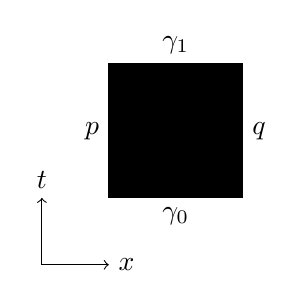
\begin{tikzpicture}[scale=.85]
	\draw[fill=\shadinga] (0, 0) rectangle (2, 2);
	\draw (1,1) node {$H_{01}$};
	\draw (1, 0) node[below] {$\gamma_0$};
	\draw (0, 1) node[left] {$p$};
	\draw (1, 2) node[above] {$\gamma_1$};
	\draw (2,  1) node[right] {$q$};	
	\draw[->] (-1, -1)--(-1, 0) ;
	\draw[->] (-1, -1)--(0,-1);
	\draw (-1,  0) node[above] {$t$};
	\draw (0, -1) node[right] {$x$};
	\end{tikzpicture}}
Notice that a homotopy between paths is nothing more than a map between $[0,1]\times [0,1]\to X$, where coordinate gives the homotopy parameter $t$ and the other one represents the path parameter $x$. The left and right portions of the square are mapped to the mutual endpoints of $\gamma_i$, and the top and bottom edges are the maps $\gamma_i$. \\

\begin{claim}
	Path homotopy is an equivalence relation on paths from $p$ to $q$. For each equivalence class of paths, we will write $[\gamma]$, the \emph{homotopy class of $\gamma$}
\end{claim}
\begin{proof}
We'll need to check the three properties of an equivalence relation. In order to do this, we'll have to construct homotopies between paths, and this proof serves as an introduction to the intuition afforded by the diagrammatic representation of path homotopies. \\
\smarginnotel{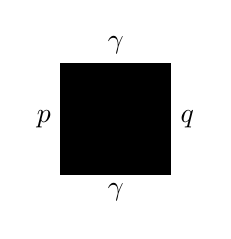
\begin{tikzpicture}[scale=.7]
	\draw[fill=\shadinga] (0, 0) rectangle (2, 2);
	\draw (1, 0) node[below] {$\gamma$};
	\draw (0, 1) node[left] {$p$};
	\draw (1, 2) node[above] {$\gamma$};
	\draw (2,  1) node[right] {$q$};	
	\draw[dashed] (0, .3)--(2, .3);
	\draw (1, .3) node[above] {$\gamma$};
	\end{tikzpicture}}We first need to show that the relation is \emph{reflexive.}
Let $\gamma_0: I\to X$ be any path. We can define the constant homotopy $H(x,  t)=\gamma(x)$ for all $t$, which is a homotopy between $\gamma$ and itself. In the diagram in the right, the dashed line and label indicates that the homotopy restricted to the dashed line gives us the path $\gamma$ in $X$.  \\

Next, we'll check that the relation of homotopy is \emph{symmetric.} \smarginnotel{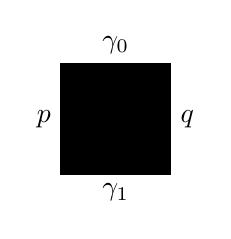
\begin{tikzpicture}[scale=.7]
	\draw[fill=\shadinga] (0, 0) rectangle (2, 2);
	\draw (1, 0) node[below] {$\gamma_1$};
	\draw (0, 1) node[left] {$p$};
	\draw (1, 2) node[above] {$\gamma_0$};
	\draw (2,  1) node[right] {$q$};
	\draw (1,1) node {\scalebox{1}[-1]{$H_{01}$}};
	\end{tikzpicture}} Suppose that $H_{01}(x,  t)$ is a homotopy between $\gamma_0$ and $\gamma_1$. Then we can define the \emph{reverse homotopy} \[H_{10}(x, t):=(x, 1-t)\] which is a homotopy between $\gamma_1$ and $\gamma_0$. In the diagram, the reflected text is suppose to tell us that the domain of the homotopy has been precomposed with a reflection map. \\

Finally, we need to check\emph{ transitivity.}\smarginnotel{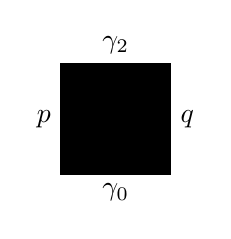
\begin{tikzpicture}[scale=.7]
	\draw[fill=\shadinga] (0, 0) rectangle (2, 2);
	\draw (1, 0) node[below] {$\gamma_0$};
	\draw (0, 1) node[left] {$p$};
	\draw (1, 2) node[above] {$\gamma_2$};
	\draw[dashed] (0,1) -- (2,1);
	\draw (2,  1) node[right] {$q$};
	\draw (1, .5) node {$H_{01}$};
	\draw (1, 1.5) node {$H_{12}$};
	\end{tikzpicture}} Suppose that $H_{01}(x,  t)$ is a homotopy between $\gamma_0$ and $\gamma_1$,  and $H_{12}(x,  t)$ is a homotopy between $\gamma_1$ and $\gamma_2$. Then define a new homotopy $H_{02}$ by 
		\[
			H_{02}(x,  t)=\left\{\begin{array}{cc}
			                     	H_{01}(x, 2t) & t\in [0, 1/2]\\
			                     	H_{12}(x, 2t-1) & t\in (1/2,  1]
			                     \end{array}\right. .
		\]
		You should check that this gives us an honest continuous homotopy between $\gamma_0$ and $\gamma_1$. In the diagram on the right, we see that our new homotopy is constructed by gluing together the domains of our old homotopies together. 

\end{proof}


\end{doubledtuftepage}

\begin{doubledtuftepage}[Concatenation and Homotopy]
We'll now look at how we can assemble loops together on a space. Given two loops, we can create a new loop which goes through each of the original loops at double speed. 
\begin{definition}
	Let $\gamma_0,  \gamma_1$ be two loops with base point $p$. Then we define the \emph{composition loop} to be piecewise composition \smarginnotel{\includegraphics[]{fundamental_pathcomposition}}
	\begin{align*}
	\gamma_0\cdot \gamma_1: [0, 1]\to& X\\ 
	 x\mapsto&\left\{\begin{array}{cc}
	                 	\gamma_0(2x) & x\in[0,  1/2]\\
	                 	\gamma_1(2x-1) & x\in (1/2,  1]
	                 \end{array}
 \right. 
	 \end{align*}
	 which is again a loop that starts with base point $p$.
\end{definition}
Unfortunately, it is almost never the case that loop composition is an associative operation on the nose.
\[(\gamma_0\cdot \gamma_1)\cdot \gamma_2\neq \gamma_0\cdot(\gamma_1\cdot \gamma_2)\] However, we'll be able to show that loop composition descends to an operation on homotopy classes of loops, and that the operation of loop composition is associative on these equivalence classes. One way of stating this is that the operation of composition fails to be associative up to a factor of homotopy.  
\begin{claim}
	Suppose that $\gamma_0\sim \gamma_1$ are two path homotopic loops,  and $\beta_0\sim \beta_2$ is another pair of homotopic loops. Then $\gamma_0\circ\beta_0 \sim \gamma_1\circ \beta_1$. In particular,  \[[\gamma]\cdot [\beta]:=[\gamma\cdot \beta],\]
	does not depend on choice of representatives.
\end{claim}
\begin{proof}

	We just need to exhibit 	\smarginnote{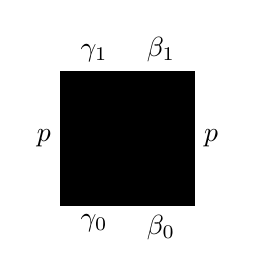
\begin{tikzpicture}[scale=.85]
		\draw[fill=\shadinga] (0, 0) rectangle (2, 2);
		\draw[dotted] (1, 0)--(1, 2);
		\draw (1.5,  0) node[below] {$\beta_0$};
		\draw (1.5,  2) node[above] {$\beta_1$};
		\draw (.5, 0) node[below] {$\gamma_0$};
		\draw (0, 1) node[left] {$p$};
		\draw (.5, 2) node[above] {$\gamma_1$};
		\draw (2,  1) node[right] {$p$};
		\draw (.5, 1) node {$H^\gamma_{01}$};
		\draw (1.5, 1) node {$H^\beta_{01}$};
		\end{tikzpicture}}a homotopy between  $\gamma_0\cdot \beta_0$ and $\gamma_1\cdot \beta_1$. Let $H^\gamma_{01}$ be the homotopy between the $\gamma_i$, and $H^\beta_{01}$ be the homotopy between the $\beta_i$. Define a new homotopy $H(x, t)$ be the piecewise composition:
	\[H(x, t)=\left\{ \begin{array}{cc} H^\gamma_{01}(2x, t) & x\in [0, 1/2]\\ H^\beta_{01} (2x-1, t) & x\in (1/2, 1]\end{array}\right.\]
	This homotopy can be visualized on the left as the associated composition of the homotopy domains. 

\end{proof}

\begin{claim}
	The composition rule is associative on homotopy equivalence classes of loops.
\end{claim}
\begin{proof}
	We need to exhibit the homotopy \[(\gamma_0\cdot \gamma_1)\cdot \gamma_2)\sim\gamma_0\cdot (\gamma_1\cdot \gamma_2)\] The difference between these two composition is only in the speeds which they trace out their respective paths.  The first composition goes through $\gamma_0$ and $\gamma_1$ at 4x speed,  and then $\gamma_2$ through double speed.   
	If we look at the second composition we instead draw $\gamma_0$ at double speed,  and $\gamma_1,  \gamma_2$ at 4x speed. \\
	In order to give a homotopy between these two composition, we merely need to reparameterize the domains to change drawing speed.\\
  Define the following homotopy between $(\gamma_0\cdot \gamma_1)\cdot \gamma_2)$ and $\gamma_0\cdot (\gamma_1\cdot \gamma_2)$. 
  \[H(x,  t)=\left\{\begin{array}{cc} 
                    	\gamma_0(4/(1+t) x) & x\in [0, (t+1)/4)\\
                    	\gamma_1(4(x-(1+t)/4))& x\in [(t+1)/4,  (t+2)/4)\\
                    	\gamma_2(4/(2-t)( x- (t+2)/4))& x\in [(t+2)/4,  1]
                    \end{array}\right.\]
	This homotopy is given by a really nasty function, and it is much easier 
\smarginnotel{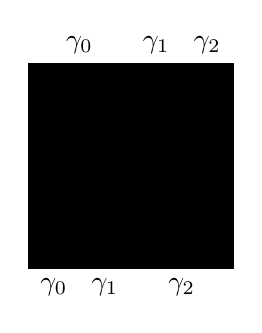
\begin{tikzpicture}[scale=1.3]
	\draw[fill=\shadinga] (0, 0) rectangle (2, 2);
	\draw[dashed] (1, 0)--(1.5, 2);
	\draw[dashed] (.5,  0)--(1,  2);
	\draw (.25, 0) node[below] {$\gamma_0$};
	\draw (.75, 0) node[below] {$\gamma_1$};
	\draw (1.5,  0) node[below] {$\gamma_2$};
	\draw (.5,  2) node[above] {$\gamma_0$};
	\draw (1.25,  2) node[above] {$\gamma_1$};
	\draw (1.75,  2) node[above] {$\gamma_2$};
\end{tikzpicture}}
	to see what this homotopy does by looking at the associated diagram of the domain. The bottom and top of the rectangle correspond to our two composition tracing out the loop $\gamma_0\cdot \gamma_1\cdot \gamma_2$ at different rates. . Each region of the rectangle corresponds to a constant homotopy between $\gamma_i$ and itself.  The diagonal stripe in the rectangle shows that there is a simple reparameterization of the domain that makes these compositions homotopic.
\end{proof}

\end{doubledtuftepage}
\begin{doubledtuftepage}[Making the Fundamental Group]
We'll now assemble the operation of loops into an algebraic object.  
	\begin{definition}
		Let the \emph{fundamental group} $(\pi_1(X, p), \cdot) $ be the set of homotopy classes of loops based at $p$ in $X$, with operation $\cdot$ given by loop composition. 
	\end{definition}
We already know that $\pi_1(X, p)$ has an associative product on it; the goal of this section is to prove that this is a group. 
\begin{claim}
	The constant loop $1_{x_0}$ has the property that
	\[[1_{x_0}]\cdot [\gamma]=[\gamma]\cdot [1_{x_0}]=[\gamma]\]
	for any loop $\gamma$ based at $x_0$. 
\end{claim}
\begin{proof}
	We use the fact that the constant loop can be reparameterized to any length that we choose. We define the homotopy as follows:
	\[
		H(x,  t)=\left\{\begin{array}{cc}
		                	x_0 & x\in [0, (1-t)/2)\\
		                	\gamma((2-t)(x-(1-t)/2)) & x\in [(1-t)/2,  1]
		                \end{array}\right.
	\]
	Again,  easier to represent with a picture. 
\smarginnotel{\begin{tikzpicture}[scale=1]
	\draw (0, 0) rectangle (2, 2);
	\draw[dotted] (1, 0)--(0, 2);
	\draw (1.5,  0) node[below] {$\gamma$};
	\draw (.5,  0) node[below] {$x_0$};
	\draw (1,  2) node[above] {$\gamma$};
	\draw[->] (-1, -1)--(-1, -.5) ;
	\draw[->] (-1, -1)--(-.5,-1);
	\draw (-1,  -.5) node[above] {$t$};
	\draw (-.5, -1) node[right] {$x$};
\end{tikzpicture}}

\end{proof}

\begin{claim}
	Suppose that $\gamma(t)$ is a loop. Define $\gamma^{-1}$ to be the loop $\gamma(-t)$. Then 
	\[[\gamma]\cdot[\gamma^{-1}]=[1_{x_0}]\]
\end{claim}
\begin{proof}
	We need to exhibit a homotopy from the loops $\gamma$ and $\gamma^{-1}$ to the constant loop. A formula for this homotopy is 
	\[
		H(x,  t)=\left\{\begin{array}{cc}
		                	\gamma(2x) & x\in [0,  (1-t)/2)\\
		                	\gamma(t) & x\in [(1-t)/2, (1+t)/2)\\
		                	\gamma(1-2x) & x\in  [(1+t)/2,  1]
		                \end{array}\right.
	\]
	Which is,  as usual ,  easier to visualize as a picture instead of a piecewise function. 
\smarginnotel{	\begin{tikzpicture}[scale=1]
	\draw (0, 0) rectangle (2, 2);
	\draw[dotted] (1, 0)--(0, 2);
	\draw (1.5,  0) node[below] {$\gamma^{-1}$};
	\draw (.5,  0) node[below] {$\gamma^{\;}$};
	\draw (1,  2) node[above] {$x_0$};
	\draw[dotted] (1, 0)--(2, 2);
	\draw[->] (-1, -1)--(-1, -.5) ;
	\draw[->] (-1, -1)--(-.5,-1);
	\draw (-1,  -.5) node[above] {$t$};
	\draw (-.5, -1) node[right] {$x$};
\end{tikzpicture}}

\end{proof}

The three claims that we made above prove that $\pi(X,  x_0)$ is a group. 
\begin{definition}
	Let $\beta$ be a path in $X$ connecting $x_0$ to $x_1$. Define the \emph{change of base point map} $F_\beta: \pi(X,  x_1)\to \pi(X,  x_0)$ as follows. Suppose that $\gamma$ is a path that has endpoints at $x_1$. Then let 
	\[F_\beta(\gamma):=(\beta\cdot \gamma\cdot \beta^{-1})\].
	This map is only dependent on the homotopy class of $h$. 
\end{definition}
\begin{claim}
	The change of base point map is a group homomorphism. 
\end{claim}
\begin{proof}
	We need to prove that the map preserves the group composition law. Here is a picture why!
	\vspace{4cm}
\end{proof}

\begin{claim}
	Suppose that $X$ is path connected. Let $x_0,  x_1\in X$ be two points in $X$. Then $\pi(X,  x_0)$ is isomorphic to $\pi(X,  x_1)$. 
\end{claim}
\begin{proof}
	Since $X$ is connected,  it is clear that there is path $\beta$ with endpoints $x_0$ and $x_1$. Check that the change of base point map is in fact an isomorphism of groups by composing it with the reverse change of base point map. 
\end{proof}

\end{doubledtuftepage}

\begin{claim}
	Suppose that $X$ and $Y$ are two different space,  and $f: X\to Y$ is a continuous function. Then there is an induced group homomorphism $f_*: \pi(X,  x_0)\to \pi(Y,  f(x_0))$. 
\end{claim}
\begin{proof}
	Using a function $f: X\to Y$,  we can take loops in $X$ and get loops in $Y$ as follows. Let $\gamma: [0, 1]\to X$ be a loop. Define 
	\[f_*(\gamma)=f\circ\gamma:[0, 1]\to Y.\]
	We can check that if $\gamma_0 \sim \gamma_1$,  then it is the case that $f_*(\gamma_0)\sim f_*(\gamma_1)$. This is because if $H(x,  t)$ is a homotopy between $\gamma_0$ and $\gamma_1$,  then $f(H(x,  t))$ is a homotopy between $f_*(\gamma_0)$ and $g_*(\gamma_1)$. \\
	Finally,  we need to check that $f_*$ respects the group operation,  that is 
	\[f_*(\gamma_0\circ \gamma_1)=f_*(\gamma_0)\circ f_*(\gamma_1)\]
\end{proof}

\begin{claim}
	Suppose that $f: X\to Y$ and $g: Y\to Z$ are two continuous maps. Then 
	\[g_*\circ f_*=(f\circ g)_*\]
\end{claim}



\begin{theorem}
	The fundamental group of the circle is $\Z$. 
\end{theorem}
\begin{proof}
	To come later in this class. But the idea is that the number of times that a loop winds around the origin tells you what number to map every loop to. 
\end{proof}

\subsection{Van Kampen's Theorem}
We would like a way to compute the fundamental group of a space $X=A\cup B$ in terms of its components $A$ and $B$. As with homology, we expect the fundamental group of this thing to be related to the fundamental group of their intersection. 
\begin{definition}
Let $G, H$ be two groups. The \emph{free product} of $G$ and $H$ is the unique group $G*H$ with maps $i:G\to G*H $, and $j: H\to G*H$ such that for any group $A$ and maps $f: G\to A$ and $g: H\to A$, there exists a unique map $\phi: G*H\to A$ such that the following diagram commutes:
\[
\begin{tikzcd}
G\arrow{d}{i} \arrow{dr}{f}\\  G*H \arrow[dashed]{r}{\phi} & A\\ H\arrow{u}{j} \arrow{ur}{h}
\end{tikzcd}
\]
\end{definition}

\begin{theorem}
Let $A$, $B$ be path connected topological spaced. Let $A\vee B$ be the \emph{wedge sum} of $A$ and $B$. Then $\pi_1(A\vee B)=\pi_1(A)*\pi_1(B).$
\end{theorem}

\section{Knot Group}
\subsection{Given as a Braid}
Here is one method for computing the fundamental group of the knot complement. Let $\beta$ be a braid which closes to $K$. Our intuition for computing the fundamental group of the knot complement will be as follows: first, think of the space $\S^3\setminus K$ as the union of two donuts where one donut contains the braid. Then cut this braid containing donut into a cylinder. Now, understand how the braid inside of the donut gives relations to the generators of the fundamental group of this cylinder. 
\[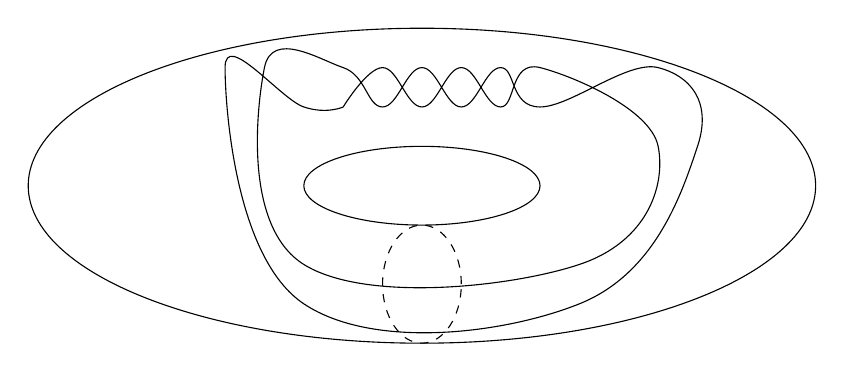
\begin{tikzpicture}[scale=.5]
\draw  plot[smooth, tension=.7] coordinates {(-3,2) (-2,3) (-1,2) (0,3) (1,2) (2,3) (5,1) (3,-2) (-4,-2) (-5,3) (-3,3) (-2,2) (-1,3) (0,2) (1,3) (2,2) (5,3) (6,1) (3,-3) (-4,-3) (-6,3) (-4,2) (-3,2)};
\draw  (-1,0) ellipse (3 and 1);
\draw  (-1,0) ellipse (10 and 4);
\draw[dashed]  (-1,-2.5) ellipse (1 and 1.5);
\end{tikzpicture}\]

Now, to make this idea rigorous, we use Van Kampen's theorem on the following decomposition. We work in cylindrical coordinates. Assume that the knot is from the closure of a braid $\beta$ on $n$ strings, and is given in such a way so that the orientation of the knot aligns with $\theta$ from our cylindrical coordinates. Furthermore, assume the whole knot is contained in the donut $(r-2)^2+z^2\leq 1$, and assume that the braid $\beta$ is contained in the portion of the torus $\theta\in [0, 180]$, so the remainder of the knot is just lines of constant $r, \theta$ values. Then we decompose the space into two parts:
\begin{itemize}
\item The first part $A$ of the space contains the braid (and a little strip for good luck.) This is the union of the cylinder $(0<\theta<2\pi, (r-1)^2+z^2<1$, and a small strip-- an open neighborhood of the curve $r=1, z=0$. Here is a drawing of the set $A$.
\[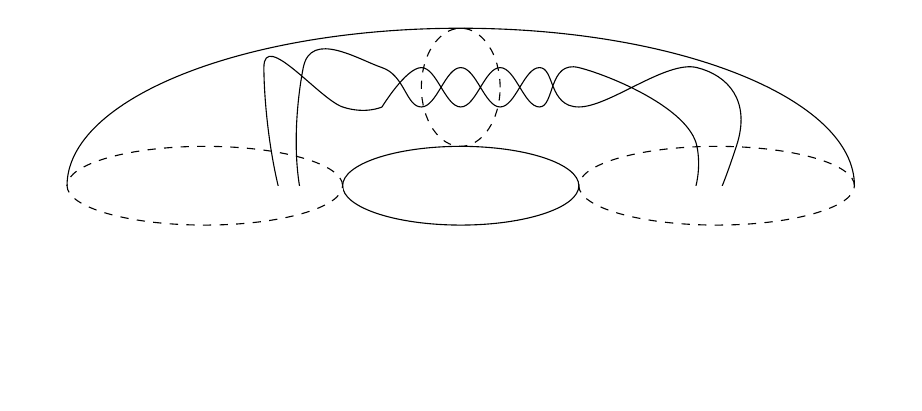
\begin{tikzpicture}[scale=.5]
\draw  plot[smooth, tension=.7] coordinates {(-3,2) (-2,3) (-1,2) (0,3) (1,2) (2,3) (5,1) (3,-2) (-4,-2) (-5,3) (-3,3) (-2,2) (-1,3) (0,2) (1,3) (2,2) (5,3) (6,1) (3,-3) (-4,-3) (-6,3) (-4,2) (-3,2)};
\draw  (-1,0) ellipse (3 and 1);
\draw  (-1,0) ellipse (10 and 4);
\draw[dashed]  (-1,+2.5) ellipse (1 and 1.5);
\fill[white]  (-12,0) rectangle (-4,-5);
\fill[white] (-6,-2) rectangle (5,-5);
\fill[white](2,0) rectangle (10
,-5);
\draw[dashed]  (-7.5,0) ellipse (3.5 and 1);
\draw[dashed]  (5.5,0) ellipse (3.5 and 1);
\end{tikzpicture}\]
\item The second part $B$ is a small open neighborhood of the complement of $A$.  This is a harder set to draw, so we will not do so here. 
\end{itemize}
Clearly from definition $A\cup B=S^3\setminus K$.  Now what does the intersection of $A$ and $B$ look like? It is a hollow cylinder, with $n$ holes poked in both the top and bottom, with a little handle attached to it. \\
Now why decompose the knot into each of these three space? Because their fundamental groups are so simple. 
\begin{itemize}
\item The Fundamental group of $A$ is the free group on $n+1$ generators, where the $+1$ generator is coming from the little handle added on.  Notice that since the braid has been ``unclosed'' it is homotopically the same as the cylinder missing $n$ lines, which has a fundamental group the free group generated by loops that go around each string complement.
\item The Fundamental group so $B$ is the free group on $n$ generators. 
\item The Fundamental group of $A\cap B$ is the Free group on $(2n-1)+1$ generators. The $2n$ generators correspond to the holes poked in the bottom and top of the hollow cylinder. The $-1$ corresponds to the fact that the loop that goes around all the generators on the left is equal to the loop that goes around all the generators on the right. The $+1$ corresponds to the lucky look that we have added on. 
\end{itemize}
Now clearly, the relationships from $B$ tell us that the left side generators of $A\cap B$ are equal to the right side generators of $A\cap B$. So, the fundamental group of $A\cup B$ will be given by generators of $A$ (less the special handle) mod out relations given by the braid, which we will write as $\beta(a)$. Now how does the braid effect these generators? \\
The braid acts by automorphism on the group $F^n=\pi_1(\RR^2\setminus \{1, \ldots n\})$, by permuting the loops. In class, we proved that these automorphisms were given by 
\[\sigma_i(a_j)=\left\{\begin{array}{cc} a_j & j\neq i,i-1\\
a_j^{-1}a_{j+1}a_j & j=i\\
a_i+1 & j=i-1
\end{array}\right.
\]
\begin{example}
With the trefoil, we can use the braid word $\sigma_1^3$ which closes to the braid. The automorphisms that we get are that 
\begin{align*}
a_2=\sigma^{3}(a_2)=\sigma^2(a_1)\\
a_2=\sigma(a_1^{-1} a_2 a_1)\\
a_2=& a_1^{-1} a_2^{-1} a_1 a_1 a_1^{-1} a_2 a_1\\
a_1 a_2 a_1^{-1}= a_2^{-1} a_1 a_2
\end{align*}
These are the relations for the braid group! 
\end{example}
\subsection{Wirtinger Presentation}
The second way to compute the knot fundamental group is to do Van Kampen's theorem on every single crossing in the knot. Here is the idea for this method of computing the fundamental group.
\begin{itemize}
\item Using a planar diagram of the knot, make it so the arcs of the knot lie all in a place $z=0$, unless there is a crossing, where the string can pop up to a height of one.\\
\item Set a base point for computing the fundamental group at some negative $z$ value.\\
\item At each crossing, remove a small ball that contains the over and under crossings. \\
\[\begin{tikzpicture}

\draw  plot[smooth, tension=.7] coordinates {(-6,0) (4,0)};
\draw (-4,-3) -- (-2,-1) -- (-2,1) -- (0,3) -- (0,1) -- (3,4);
\draw  (-1,1) ellipse (4 and 4);
\node at (0,-5) {$x_0$};
\node at (-6,1) {$\alpha$};
\node at (-4,-4) {$\beta$};
\node at (4,1) {$\gamma$};
\node at (3,5) {$\delta$};
\end{tikzpicture}\]

\item Now we have a bunch of arcs connecting removed balls. Each arc gives a generator for the fundamental group.
\item Figure out what relations we add back in when we put in the balls. 
\end{itemize}
To figure out what relation we add back in, we just need to understand what the fundamental group of the sphere missing 4 points is related to the ball with two arcs removed is. If $\alpha, \beta, \gamma$ and $ \delta$ are the four loops on the boundary sphere, with base point at the bottom of the sphere, then the relation between them is given by $\alpha=\gamma^{-1}$, and $\beta=\alpha^{-1} \delta^{-1}\alpha$. This means that the added relations that we get at each crossing are that the ``through'' arc stays the same, but the under arcs are related by conjugation by the ``through'' arc. \project
\newpage

\section{A tie in to Multivariable Calculus}
While an exposition of the tools used in differential geometry (manifolds, tangent bundles and the de Rahm cohomology) is beyond the scope of these notes, some of the basic constructions of de Rahm theory can already be accessed using multivariable calculus and have relevant analogies to constructions in this course.\\
Due to the notational limits of multi variable calculus, we will strictly work in the 3 dimensional case-- however, all of these results hold equally as well in the 2-dimensional case, and with the development of the language of differential forms can be made to work on arbitrary smooth manifolds. 
\begin{definition}
	Let $U$ be a subspace of $\RR^3$. A \emph{smooth function} on $U$ is a function $f: U\to R$ which is infinitely differentiable. A \emph{smooth vector field} is a triple of smooth functions 
	\[X=\langle f, g, h\rangle.\]
	We'll denote the space of all smooth function $\Func(U)$, and the space of all smooth vector fields $\Vect(U)$. 
\end{definition}
Most of an introductory multivariable calculus course is devoted to defining a variety of tools that can be used manipulate vector fields and functions. We break these into 3 classes: products, differentials, and integrals. 

\subsection{Differentials}
One of the principle difficulties of learning multivariable calculus is finding a good framework to fit in the multitude of different derivatives that are introduced in the course. In 3 dimensions, we have no fewer than 3 different types of derivatives, each measuring different properties with different physical intuitions. We'll quickly review these different derivatives and fix the notation that we'll use for the remainder of this section. \\
The first derivative that we're introduced to in multivariable calculus is the \emph{gradient} which is defined in any dimension. The gradient inputs a smooth function $f$ and outputs a vector field $\grad f$. \footnote{Also sometimes denoted as $\nabla\cdot f.$}
\begin{align*}
\grad: \Func(U)\to& \Vect(U)\\
f\mapsto &\langle f_x, f_y, x_z\rangle 
\end{align*}
One intuition for the physical meaning of the gradient in $\RR^n$ is that it returns the vector field that points in the direction of largest increase of our vector field. This intuition tells us why, for instance, the zeros of the gradient correspond to critical points of the function $f$. \\
Given a vector field, there are two different kinds of derivatives that we can take. The first variety is the \emph{curl}, which outputs another vector field. 
\begin{align*}
\curl: \Vect(U)\to&\Vect(U)\\
\langle f, g, h\rangle \mapsto & \langle h_y-g_z, f_z-h_x, g_x-f_y\rangle
\end{align*}
The curl of a vector field is suppose to be a measure of how much rotational inertia a vector field imparts on a particle that is being moved by the vector field; the magnitude of the curl field gives the amount of energy imparted while the direction of curl field denotes the plane of rotation. \\
The second type of derivative that we can take is the \emph{divergence}, which outputs a function. 
\begin{align*}
\ddiv: \Vect(U)\to&\Func(U)\\
\langle f, g, h\rangle \mapsto& f_x+g_y+h_z
\end{align*}
Should a vector field $X$ measure the flow of a fluid, the divergence of a vector field is suppose to measure the net compression / decompression of $X$ at any given point. \\
Without more intuition, it's not possible to tell how these three operators fit together in a unified framework; however, the following 2 lemmas suggest that we should think of these in the sequence 
\[
\begin{tikzcd}
0 \arrow{r} &\Func(U)\arrow{r}{\grad} & \Vect(U) \arrow{r}{\curl} & \Vect(U) \arrow{r}{\ddiv} & \Func(U)\arrow{r} & 0 
\end{tikzcd}
\]
\begin{claim}
	The composition $\curl\circ \grad(f)=0$. 
\end{claim}
This is sometimes stated as ``every gradient vector field is conservative'' or ``every gradient  field is curl free.'' The proof of this claim is by a simple algebraic computation. 
\begin{claim}
	The composition $\ddiv \circ \curl (X)=0$. 
\end{claim}
This is sometimes stated as ``every curl field is noncompressible'' or ``every curl field is divergence free.'' Again, the proof of this claim is simply checking the definitions. \\
With these claims and the machinery built in class, we come to the somewhat remarkable observation that 
\[
\begin{tikzcd}
0 \arrow{r} &\Func^0(U)\arrow{r}{\grad} & \Vect^1(U) \arrow{r}{\curl} & \Vect^2(U) \arrow{r}{\ddiv} & \Func^3(U)\arrow{r} & 0 
\end{tikzcd}
\]
is a (co)chain complex. This chain complex is very different than those that we've defined earlier in class, as each of the chain groups has uncountable dimension. Never-the-less, it still makes sense to make the following definitions:
\begin{definition}
	Let $U$ be a subset of $\RR^3$. Define the \emph{de Rahm cohomology groups} to be the quotients 
	\begin{align*}
	H^0_{dr}(U)=\ker(\grad) && H^1_{dr}(U)=\frac{\ker(\curl)}{\im(\grad)}\\
	H^2_{dr}(U)=\frac{\ker(\ddiv)}{\im(grad)} && H^3_{dr}(U)=\frac{\Func^3(U)}{\im(\ddiv)}.
	\end{align*}
\end{definition}

\subsection{Integrals}

\subsection{Some Sample Computations}